\section{Additional Panel and local model estimation results}
\label{appx:model_results}
\subsection{Panel model estimation results}
The full list of countries used in the panel estimation includes Armenia, Australia, Austria, Belgium, Brazil, Chile, Colombia, Croatia, Czech Republic, Denmark, Finland, France, Georgia, Germany, Greece, Hong Kong, China, Hungary, Iceland, India, Ireland, Israel, Italy, Japan, Korea, Republic of, Mexico, Netherlands, New Zealand, Norway, Philippines, Poland, Portugal, Romania, Russian Federation, Singapore, Spain, Sweden, Switzerland, Thailand, Türkiye, United Kingdom and United States.
\begin{table}[!ht]
\begin{center}
\caption{In-sample panel quantile regression coefficients.}
\label{table:panel_coeffs}
\scalebox{0.6}{
\begin{tabular}{p{7cm}p{3cm}p{3cm}}
\hline
                                           & GDP growth, h=4, q=0.1, e=f & GDP growth, h=4, q=0.5, e=f \\
\hline
autoregressive                             & 0.0302                      & 0.1038***                    \\
                                           & (0.0276)                    & (0.0107)                     \\
FCyI                                       & -3.4029***                  & -2.0606***                   \\
                                           & (0.6489)                    & (0.3287)                     \\
FCI                                        & 0.2306*                     & 0.1166**                     \\
                                           & (0.1188)                    & (0.0593)                     \\
MPI                                        & 0.1012*                     & -0.0221                      \\
                                           & (0.0550)                    & (0.0275)                     \\
DSR                                        & -0.1543***                  & -0.1084***                   \\
                                           & (0.0274)                    & (0.0147)                     \\
Interest\_margin/Income\_normalized\_C\_2y & -0.1249**                   & -0.0268                      \\
                                           & (0.0559)                    & (0.0270)                     \\
Bank\_liabilities\_MC\_normalized\_C\_1y   & -0.8270***                  & -0.5366***                   \\
                                           & (0.1662)                    & (0.0803)                     \\
NPL\_ratio\_PctC\_3y                       & -0.1747***                  & -0.0424                      \\
                                           & (0.0562)                    & (0.0290)                     \\
Provisions/NPL\_C\_2y                      & 0.0231***                   & 0.0057**                     \\
                                           & (0.0044)                    & (0.0024)                     \\
RPP\_Real\_PctC\_3y                        & 3.6966***                   & 3.9197***                    \\
                                           & (0.4692)                    & (0.2543)                     \\
RRE\_Loans\_MC\_PctC\_1y                   & 1.3092***                   & 0.7058***                    \\
                                           & (0.1921)                    & (0.1395)                     \\
CPI\_C\_1y                                 & -0.1441***                  & -0.0532***                   \\
                                           & (0.0212)                    & (0.0109)                     \\
MPR\_log                                   & -0.2010***                  & -0.0307                      \\
                                           & (0.0539)                    & (0.0273)                     \\
Unemployment\_normalized                   & 1.0673***                   & 0.6037***                    \\
                                           & (0.0969)                    & (0.0451)                     \\
FX\_log\_C\_2y                             & 0.8575***                   & 0.5483***                    \\
                                           & (0.1767)                    & (0.0886)                     \\
Import\_Merchandise\_Price\_normalized     & -0.9196***                  & -0.4745***                   \\
                                           & (0.0833)                    & (0.0405)                     \\
FCyI x FCI                                 & 2.0863***                   & 0.9796**                     \\
                                           & (0.6735)                    & (0.3813)                     \\
MPI x FCyI                                 & -0.2048*                    & 0.0615                       \\
                                           & (0.1066)                    & (0.0614)                     \\
MPI x FCI                                  & -0.9881***                  & -0.3099***                   \\
                                           & (0.1947)                    & (0.0913)                     \\
N                                          & 4469.0000                   & 4469.0000                    \\
Pseudo-R2                                  & 0.1831                      & 0.2007                       \\
\hline \\
\multicolumn{3}{l}{* p<0.05,  ** p<0.01,  *** p<0.001}
\end{tabular}
}
\end{center}
\end{table}
\begin{figure}
	\centering 
	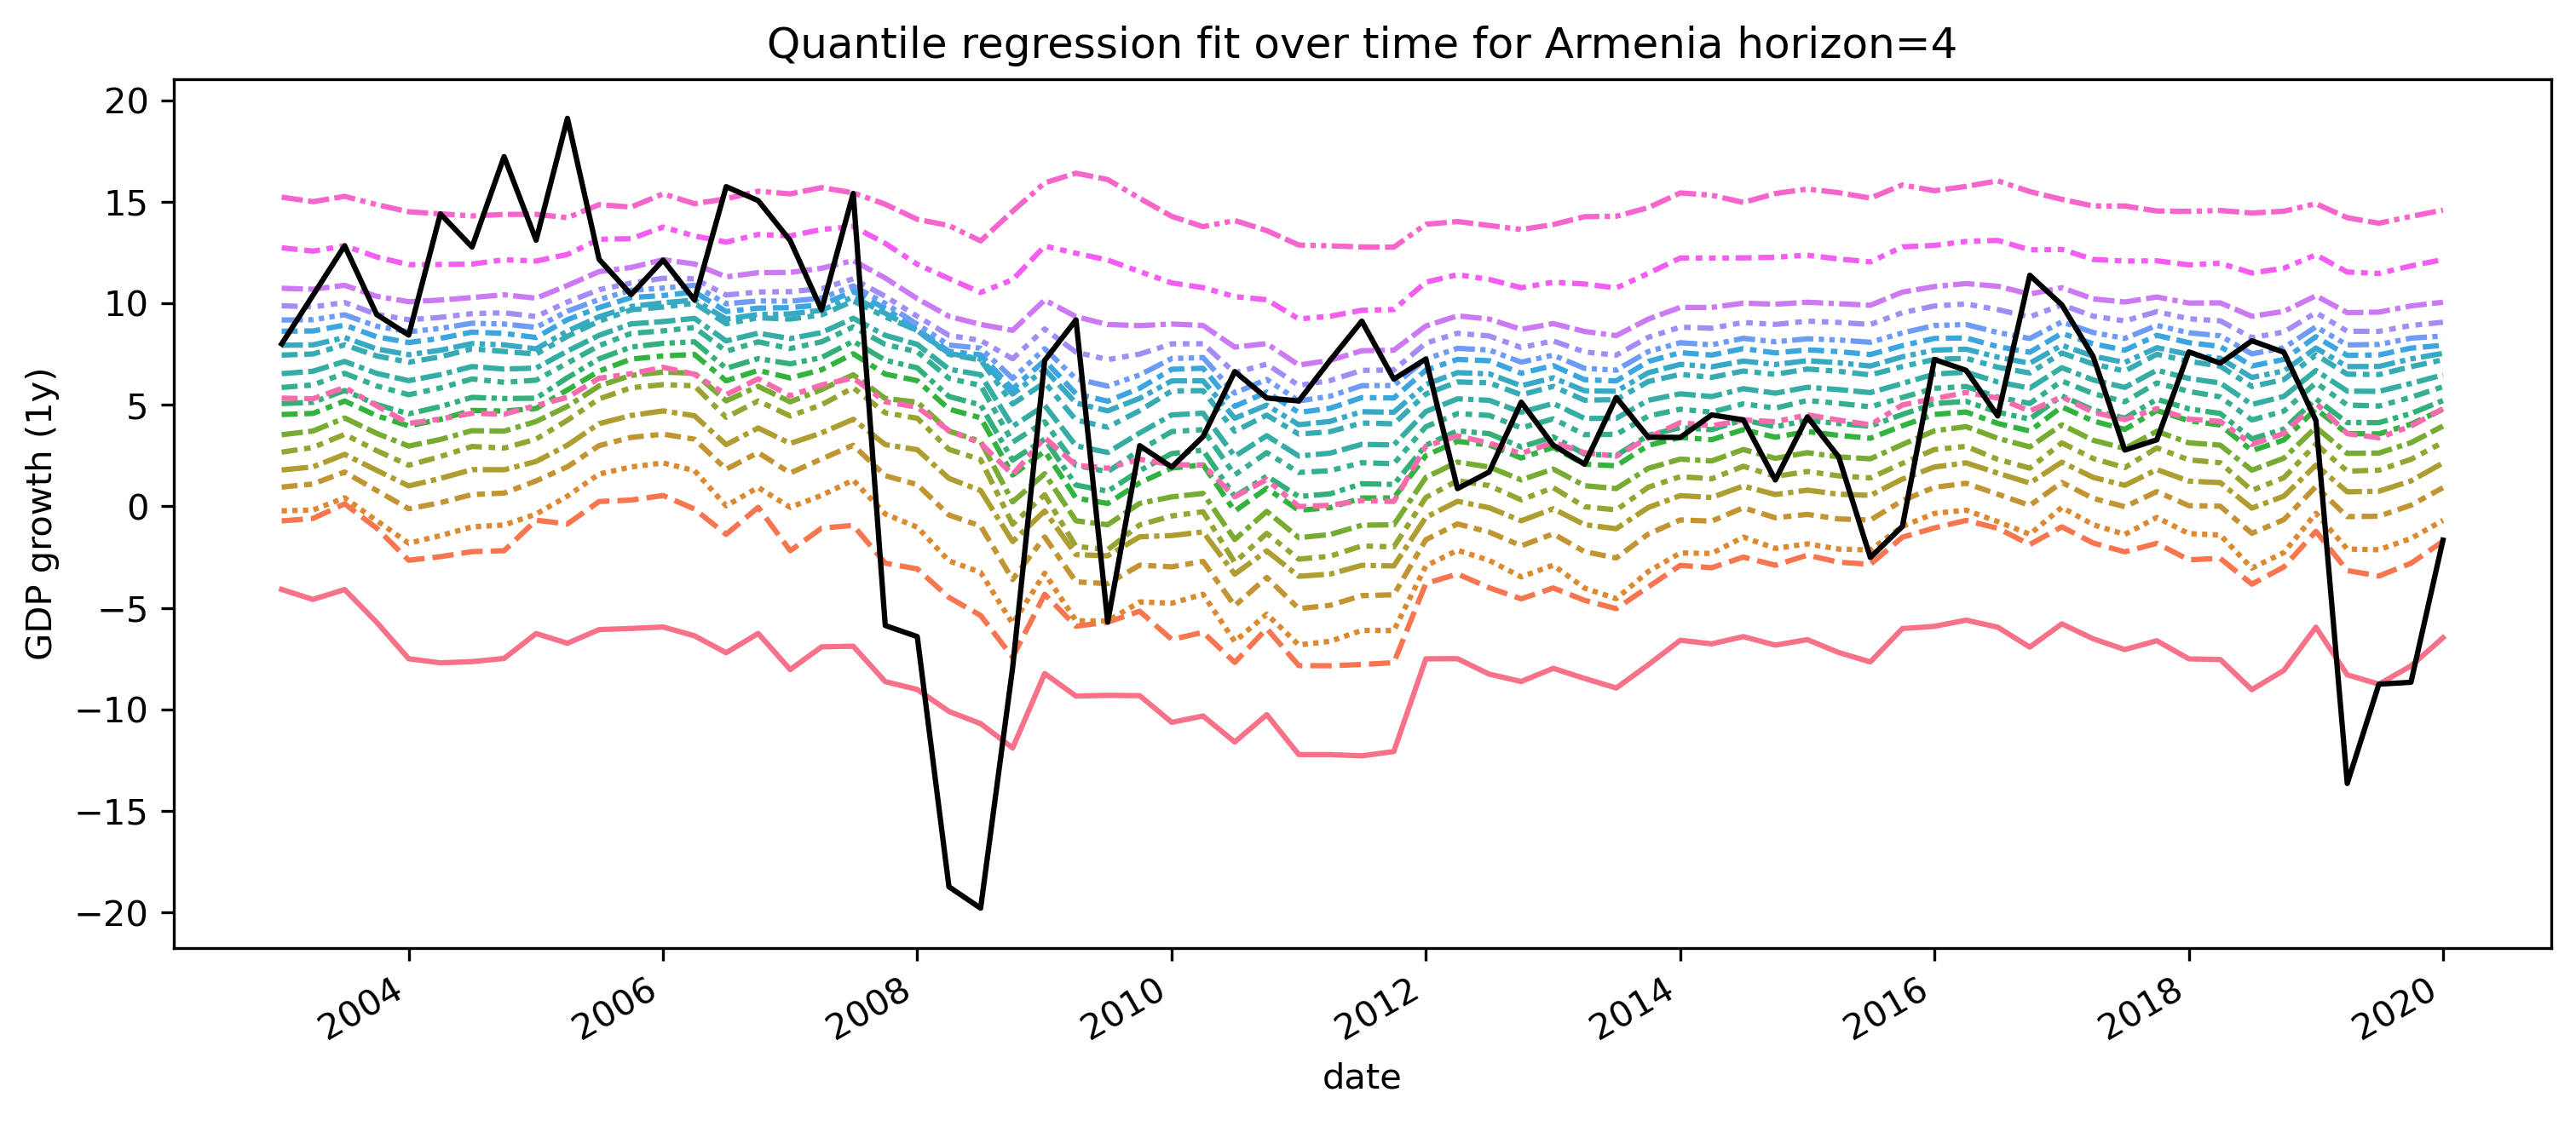
\includegraphics[width=0.45\textwidth, angle=0]{Figures/panel_qr_prediction_for_Armenia.png}	
	\caption{Panel quantile regression one year ahead fitted values of Armenia for different quantiles.} 
	\label{fig:panel_qr_prediction_for_Armenia}%
\end{figure}

In \autoref{fig:frontier_boundary} we plot the estimated median and distance-to-tail (Gap) values. We then use the Local Outlier Factor (LOF) algorithm on the data points to compute local densities for each of the points relative to their neighbors. Points with very low density are considered to be outliers (marked in red). Using this density function we derive a boundary that best describes the efficient frontier for our risk (Gap) and reward (median) pairs. Boundary points are marked in orange. By fitting a polynomial onto these points, it is possible to derive an explicit frontier function.
\begin{figure}
	\centering 
	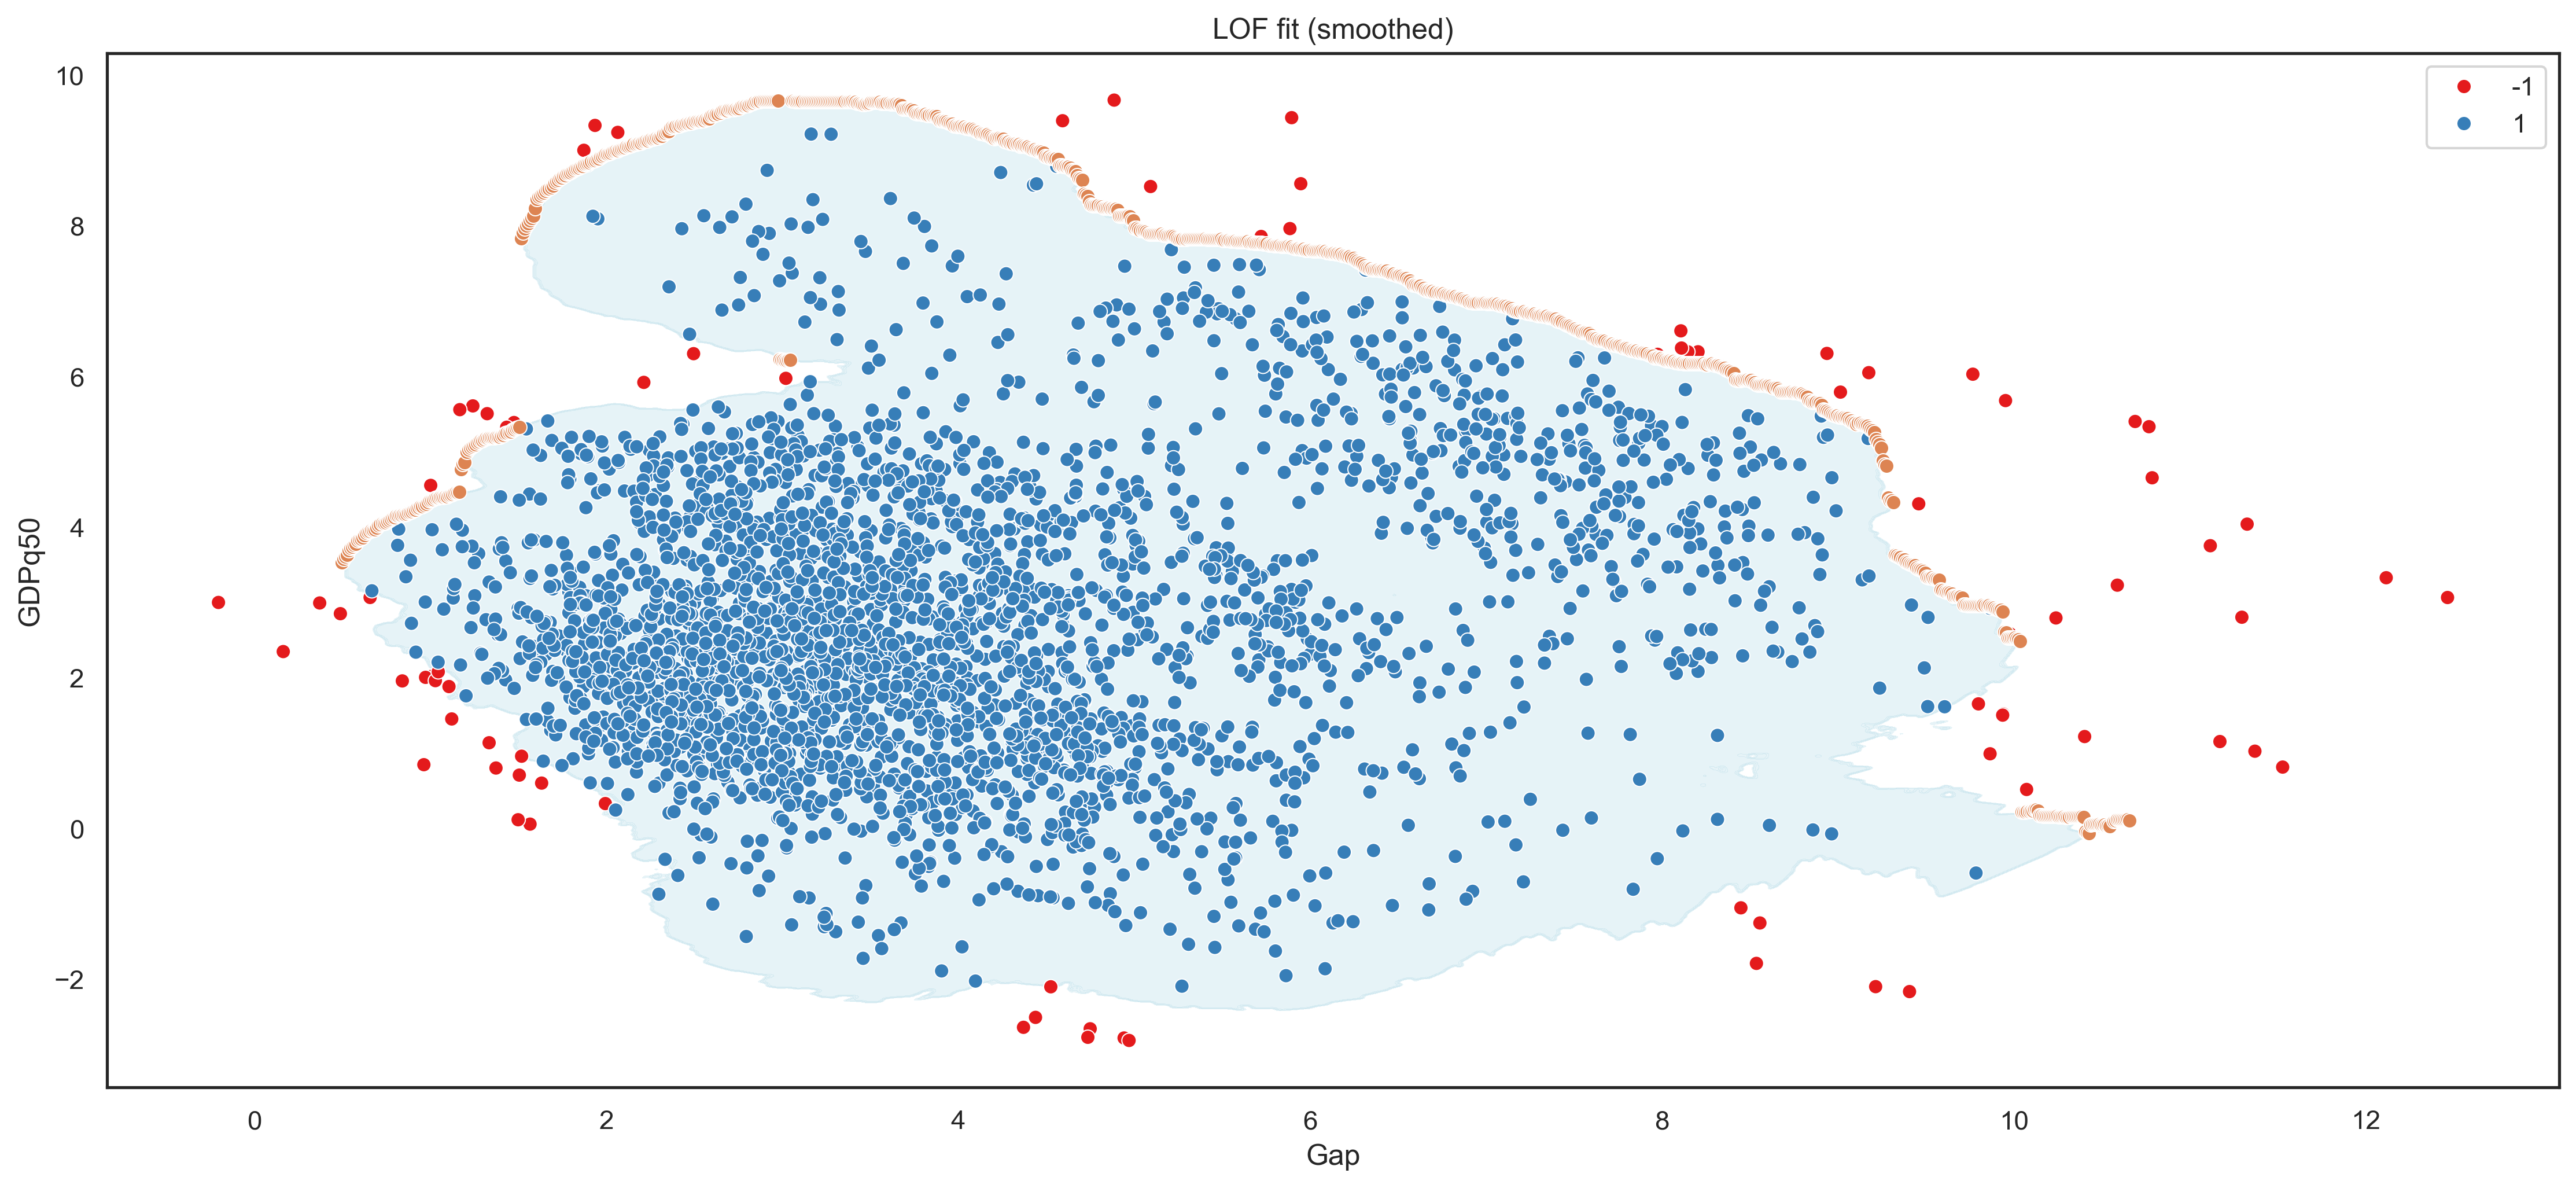
\includegraphics[width=0.45\textwidth, angle=0]{Figures/frontier_boundary.png}	
	\caption{Local Outlier Factor (LOF) boundary based on estimates from 41 countries.} 
	\label{fig:frontier_boundary}%
\end{figure}

\subsection{Local model estimation results}
\begin{table}[!ht]
\begin{center}
\caption{In-sample local quantile regression coefficients}
\label{table:local_coeffs}
\scalebox{0.6}{
\begin{tabular}{p{7cm}p{1.5cm}p{1.5cm}p{1.5cm}p{1.5cm}}
\hline
                           & GDP growth, h=4, q=0.1, e=b & GDP growth, h=4, q=0.1, e=f & GDP growth, h=4, q=0.5, e=b & GDP growth, h=4, q=0.5, e=f  \\
\hline
autoregressive             & -0.49***                    & -0.10                       & -0.41***                    & -0.19*                       \\
                           & (0.15)                      & (0.20)                      & (0.09)                      & (0.11)                       \\
const                      & -11.06**                    & 10.90                       & -1.03                       & 5.20*                        \\
                           & (4.60)                      & (7.75)                      & (3.11)                      & (2.95)                       \\
Financial Cycle Index      & 46.43**                     & -63.60*                     & 33.46**                     & -2.61                        \\
                           & (17.72)                     & (31.94)                     & (13.36)                     & (13.15)                      \\
Financial Conditions Index & -2.47                       & 4.83**                      & -2.16                       & 2.34*                        \\
                           & (1.92)                      & (2.02)                      & (1.33)                      & (1.32)                       \\
Liquidity excess           & 56.85**                     & -7.73                       & 28.59**                     & 19.38                        \\
                           & (22.58)                     & (31.87)                     & (13.36)                     & (12.43)                      \\
CAR excess\_C\_2y          & -61.56**                    & -44.55*                     & -23.07                      & -18.15                       \\
                           & (30.67)                     & (25.40)                     & (23.01)                     & (21.13)                      \\
MPI                        & -1.11**                     & 0.14                        & -0.49                       & -0.42                        \\
                           & (0.50)                      & (0.57)                      & (0.37)                      & (0.34)                       \\
FCI x FCyI                 & -4.05***                    & 7.65***                     & -1.50                       & 1.89**                       \\
                           & (1.51)                      & (1.86)                      & (0.96)                      & (0.94)                       \\
MPI x FCyI                 & -0.86*                      & 0.01                        & 0.02                        & -1.40***                     \\
                           & (0.50)                      & (0.83)                      & (0.35)                      & (0.34)                       \\
MPI x FCI                  & -1.34                       & -1.34                       & -0.52                       & 0.10                         \\
                           & (0.97)                      & (0.89)                      & (0.53)                      & (0.45)                       \\
Macroeconomic Indicator    & 21.75***                    & 8.46*                       & 19.36***                    & 11.51***                     \\
                           & (4.11)                      & (4.33)                      & (2.88)                      & (3.11)                       \\
N                          & 77.0000                     & 73.0000                     & 77.0000                     & 73.0000                      \\
Pseudo-R2                  & 0.6597                      & 0.5872                      & 0.4997                      & 0.4726                       \\
\hline \\
\multicolumn{3}{l}{* p<0.05,  ** p<0.01,  *** p<0.001}
\end{tabular}
}
\end{center}
\end{table}
\begin{figure}
	\centering 
	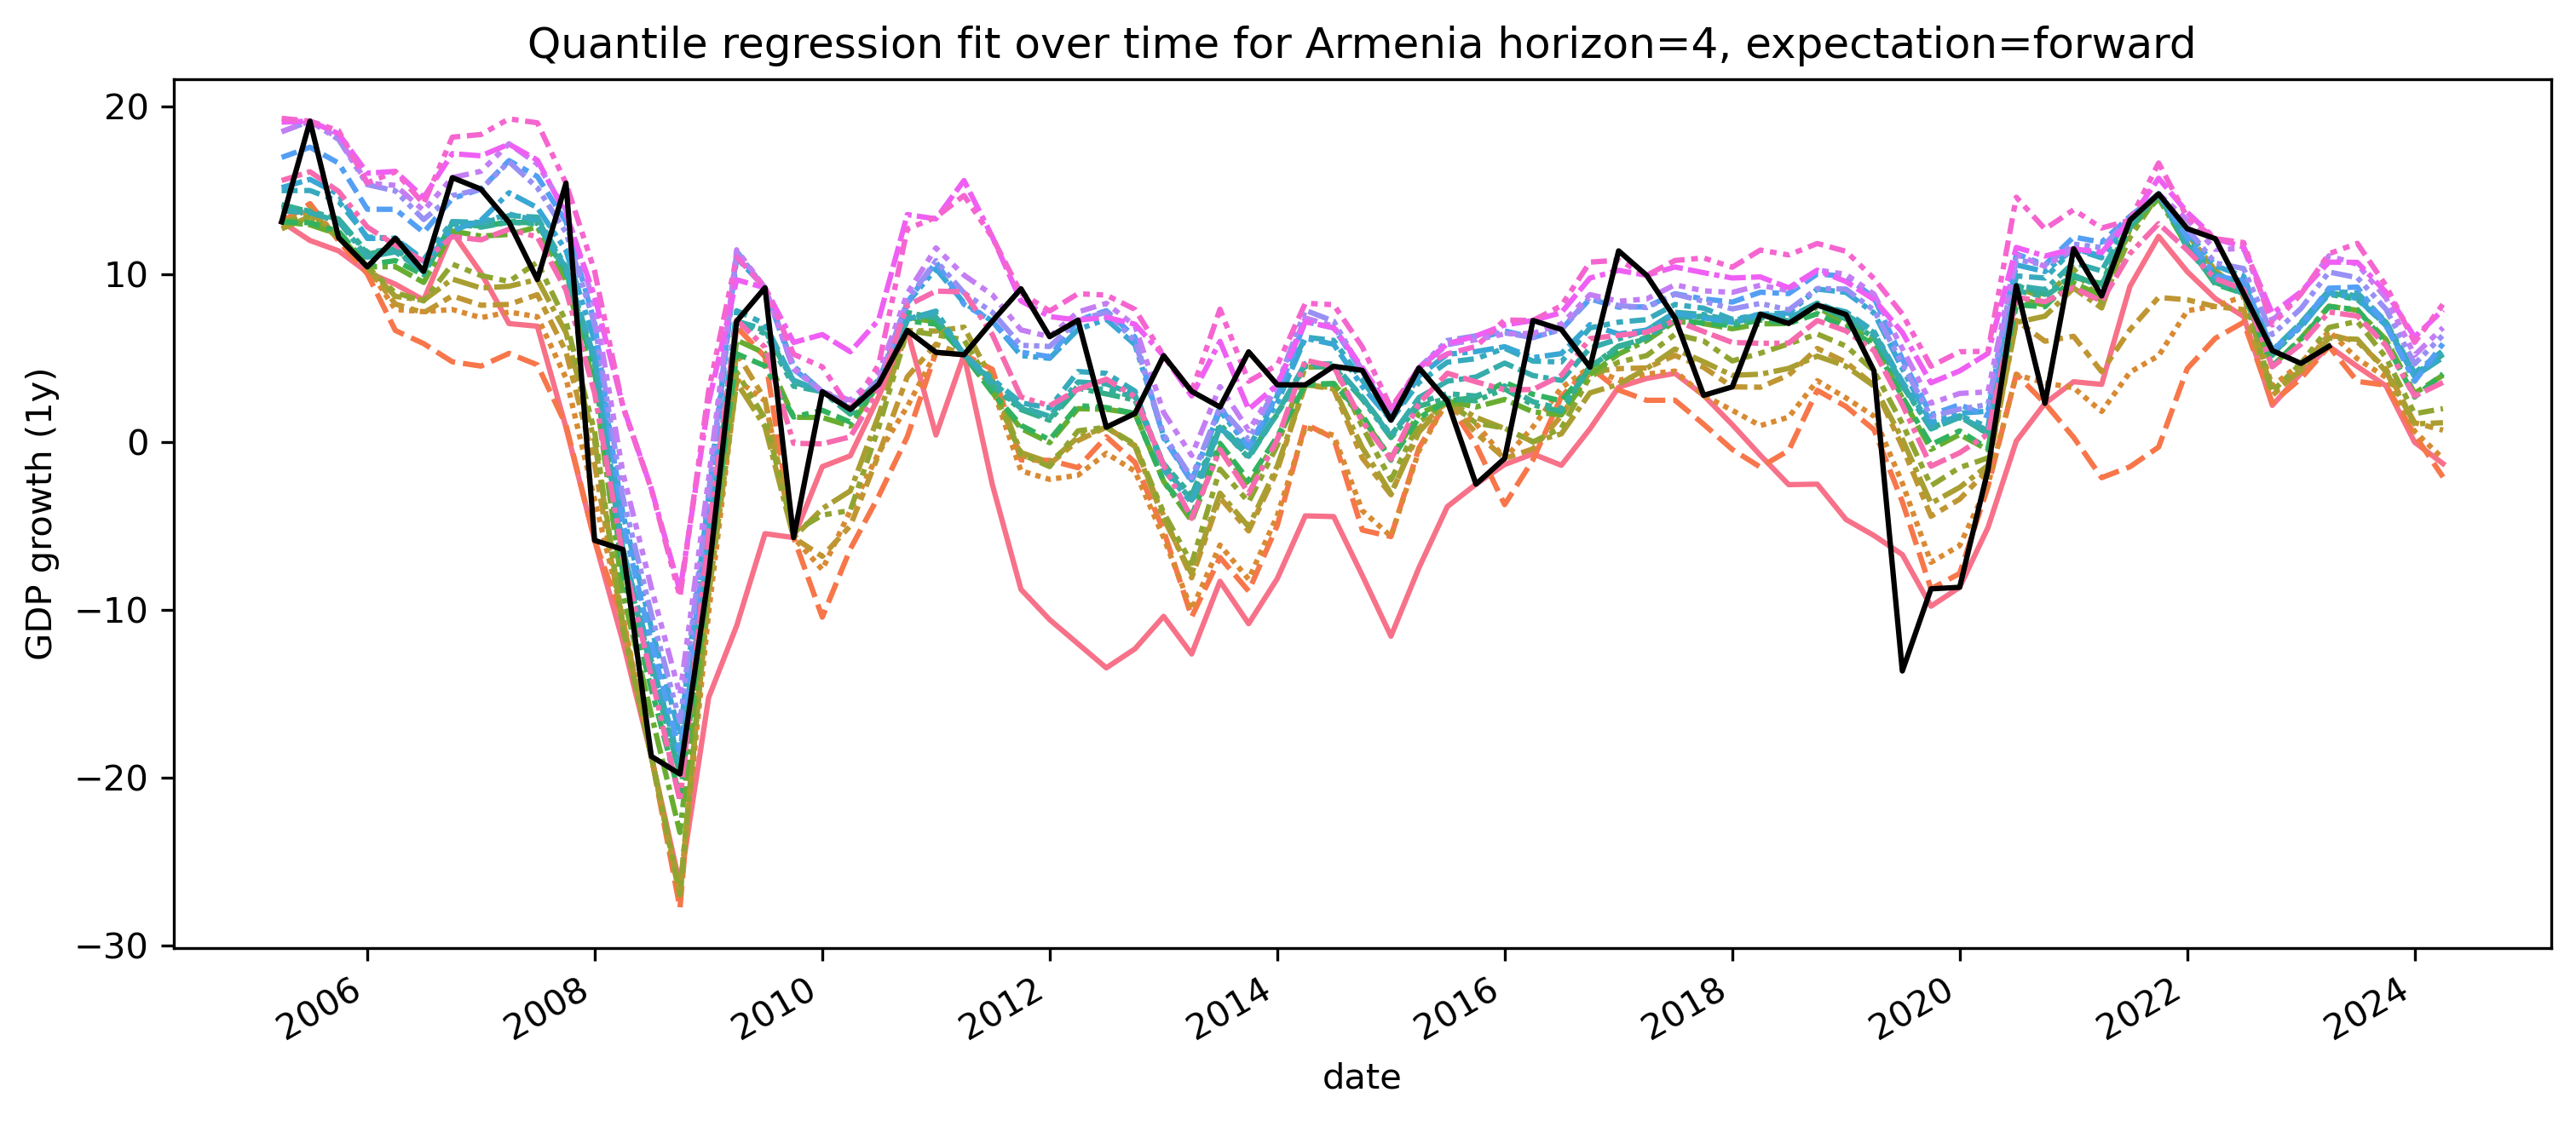
\includegraphics[width=0.45\textwidth, angle=0]{Figures/arm_qr_f_fits.png}	
	\caption{Local quantile regression one year ahead fitted values of Armenia for different quantiles.} 
	\label{fig:arm_qr_f_fits}%
\end{figure}

\autoref{fig:arm_qr_gdp_kde_dist} shows the GDP growth distribution of Armenia conditional on systemic risks in 2024Q1. Instead of using skewed t-distribution as in \autoref{fig:arm_qr_gdp_dist}, a Kernel density-based estimation is used to interpolate the quantiles. Even though it is more sensitive to the choice of the number of quantiles, it does a better job of describing the left tail of the distribution.
\begin{figure}
	\centering 
	
\includegraphics[width=0.45\textwidth, angle=0]{Figures/arm_qr_gdp_kde_dist.png}	
	\caption{Conditional GDP growth distribution using non-parametric KDE-based interpolation.} 
	\label{fig:arm_qr_gdp_kde_dist}%
\end{figure}